\documentclass[a4paper]{scrartcl}
\usepackage[czech]{babel}
\usepackage{amsmath,amssymb}
\usepackage[T1]{fontenc}
\usepackage[utf8]{inputenc}
\usepackage{bookmark}
\usepackage{hyperref}
\usepackage{dirtytalk}
\hypersetup{hidelinks}
\usepackage[normalem]{ulem}
\usepackage{multicol}
\usepackage{microtype}
\usepackage{tasks}
\usepackage{graphicx}
\usepackage{lscape}
\usepackage{enumitem}
\setlist[enumerate,1]{label=\arabic*, ref=\thesection.\arabic*}
\setlist[enumerate,2]{label=\alph*), ref=\theenumi.\alph*}
\setlist[enumerate,3]{label=\arabic*., ref=\theenumii.\arabic*}

\renewcommand{\thesection}{\Roman{section}} 

\title{Ubytovací řád a obchodní podmínky \\ {Penzion Spáleniště} }
\author{Martina Kytýrová}
%\date{}

\begin{document}
\maketitle

Tento ubytovací řád a obchodní podmínky (dále jen \say{\textbf{Ubytovací
    řád}}), který tvoří nedílnou součást smlouvy o~ubytování, stanoví
\uline{závazné podmínky přechodného ubytování a souvisejících služeb
  v~\say{Penzionu Spáleniště.}}

\section{Vymezení pojmů}

\begin{enumerate}

  \item
        Následující pojmy, psané velkými počátečními písmeny, mají
        v~Ubytovacím řádu následující význam:

        \begin{enumerate}

          \item
                \textbf{Apartmány}: společné označení pro Apartmán 1 a Apartmán 2,
                tvořící ubytovací kapacity Penzionu, jako minoritní, oddělená část
                soukromé budovy čp. 17, Spáleniště;
          \item
                \textbf{Apartmán 1}: apartmán v přízemí Penzionu, sestávající ze 2
                ložnic, kuchyně a koupelny vč. WC.
          \item
                \textbf{Apartmán 2}: apartmán v 1. patře Penzionu, sestávající
                ze~2 ložnic, kuchyně, koupelny vč. WC a~podkroví.
          \item
                \textbf{Areál}: venkovní prostory přiléhající k~Penzionu, se
                kterým tvoří jeden funkční celek; plánek, který~vymezuje část
                užívanou výhradně vlastníkem Areálu, je přílohou Ubytovacího řádu;
          \item
                \textbf{Ceník}: přehled cen ubytování (pultových, lišících se dle
                sezony) a dalších Služeb; Ceník je zásadně zveřejněn na Webu a
                v~Penzionu; ceny jsou uváděny včetně všech daní a poplatků, včetně
                DPH, je-li Ubytovatel plátce daně;
          \item
                \textbf{Host:} zájemce o ubytování i ubytovaný, jako smluvní
                strany Smlouvy, za Hosta se rovněž přiměřeně považují osoby
                ubytované či pobývající v~Penzionu společně s~Hostem-smluvní
                stranou, jejichž~ubytování či pobyt byl Penzionu nahlášen.
          \item
                \textbf{OZ:} zákon č. 89/2012 Sb., občanský zákoník, ve znění
                pozdějších předpisů;
          \item
                \textbf{Penzion} (případně \textbf{Ubytovací zařízení}): malé,
                rodinné, ubytovací zařízení poskytující ubytování v~soukromí, pod
                názvem „\emph{Penzion Spáleniště}``, provozované v~budově na
                adrese: Spáleniště č. p. 17, 51801 Dobruška;
          \item
                \textbf{Příjezdový formulář}: písemné potvrzení nástupu do
                ubytování sepisované při příjezdu Hosta; řádně vyplněný formulář
                je nezbytnou podmínkou zahájení poskytování Služeb;
          \item
                \textbf{Rezervace:} žádost o prověření dostupnosti termínu
                ubytování a návrh na uzavření Smlouvy v~rozsahu požadavku Hosta a
                zároveň označení pro vyblokování kapacit Ubytování do okamžiku
                příjezdu Hosta;
          \item
                \textbf{Služby}: ubytovací služby a případně též další související
                služby v~rozsahu a termínech stanovených Smlouvou za podmínek
                ujednaných ve Smlouvě a~stanovených v~tomto Ubytovacím řádu;
          \item
                \textbf{Smlouva}: smlouva o ubytování ve smyslu ust. § 2326 OZ,
                uzavíraná mezi Ubytovatelem a Hostem s~předmětem poskytnutí
                Služeb; podrobnosti týkající se způsobu uzavírání Smlouvy
                stanovuje Ubytovací řád v~čl. V.; v~případě rozporu podmínek
                Služeb mezi tímto ubytovacím řádem a~smlouvou mají přednost
                ustanovení Smlouvy.
          \item
                \textbf{Ubytovatel}: Martina Kytýrová, IČ: 638 24~647, se sídlem:
                Spáleniště 17, 518~01, Dobruška;
          \item
                \textbf{Web}: internetové stránky Penzionu dostupné z
                \href{http://www.penzionspaleniste.cz/}{www.penzionspaleniste.cz}.
        \end{enumerate}
\end{enumerate}

\section{Ubytovací řád}

\begin{enumerate}

  \item
        Základní podmínky a pravidla ubytování v Penzionu jsou následující:

        \begin{enumerate}

          \item
                minimální doba pobytu 2 noci;
          \item
                začátek ubytování \textbf{(check-in) od 15:00 do 20:00 hod.}
                prvního dne ubytování; mimo uvedenou dobu po předchozí domluvě
                s~Ubytovatelem;
          \item
                ukončení ubytování \textbf{(check-out) nejpozději do 10 hod.}
                posledního dne ubytování, není-li dohodnuto jinak; čas je dodržen,
                pokud jsou v~této době vráceny všechny klíče od Apartmánu a
                Apartmán je vyklizen od věcí Hosta; pokud Host bez předchozí
                dohody s~Ubytovatelem čas ukončení ubytování poruší, je Ubytovatel
                oprávněn účtovat tomuto hostu cenu ve výši dalšího jednodenního
                ubytování v~Penzionu;
          \item
                ubytování a přechovávání psů, koček a všech dalších zvířat
                \textbf{není dovoleno.}
        \end{enumerate}
  \item
        Další pravidla chování a pohybu Hostů v~Penzionu jsou určena
        následovně:

        \begin{enumerate}

          \item
                Hosté jsou povinni dodržovat Ubytovací řád, bezpečnostní a
                hygienické předpisy, zachovávat pravidla občanského soužití a
                nečinit nic, co by mohlo ohrozit bezpečnost osob a majetku,
                narušit pořádek, čistotu a klid, zejména platí:

                \begin{enumerate}

                  \item
                        noční klid v době \textbf{od 22:00 do 6:00 hod. každý den} bez
                        výjimky;
                  \item
                        \textbf{striktní zákaz kouření} ve veškerých vnitřních prostorech
                        Penzionu (pro~kuřáky jsou vyhrazena konkrétní označená místa
                        v~Areálu); zákaz rozdělávání ohně ve vnitřních prostorách a mimo
                        vyhrazená místa v Areálu; po použití venkovního grilu a~ohniště je
                        Host povinen topeniště bezpečně uhasit.
                  \item
                        zákaz přechovávání zbraní, držení či přechovávání nebezpečných
                        chemických, omamných nebo psychotropních látek a~jedů;
                  \item
                        zákaz zásahů do elektrické sítě a vodovodní instalace; hostům není
                        povoleno používat vlastní elektrické spotřebiče s výjimkou
                        elektrických spotřebičů sloužících osobní hygieně (holící strojky,
                        vysoušeče vlasů) či běžných nabíjecích nástrojů (osobní počítače,
                        mobilní telefony, fotoaparáty apod.); nejsou povoleny vařiče,
                        rychlovarné konvice, přímotopy;
                  \item
                        Host je povinen uzavřít okna, vodovodní kohoutky a zhasnout světla a
                        uzamknout Apartmán při odchodu z~Apartmánu.
                \end{enumerate}

          \item
                Hosté udržují v~Ubytovacím zařízení i jeho okolí čistotu
                a~chovají~se~šetrně k~jeho zařízení, které užívají pouze přiměřeně,
                pro stanovený účel. Bez předchozího souhlasu Ubytovatele není
                dovoleno přemisťovat a činit jakékoli zásahy do zařízení či staveb a
                prostor Penzionu/Areálu;
          \item
                Pohyb Hostů je povolen pouze v~jim vymezených prostorech, nikoli
                v~prostorách vyhrazených vlastníkovi Areálu; veškerý pohyb v Areálu
                (včetně používání herních prvků) je Hosty uskutečňován na~vlastní
                nebezpečí a náklady; zakazuje se ponechávat nedospělé děti bez
                dozoru osoby starší 18 let; vážnější úrazy či zranění vzniklá
                v~Penzionu/Areálu jsou obratem hlášena Ubytovateli;
          \item
                Ubytovatel je oprávněn odepřít ubytování osobám postiženým
                (podezřelým na výskyt) infekčními nebo parazitárními chorobami,
                osobám s nařízeným zvýšeným zdravotní dozorem, karanténou
                či~izolací;
          \item
                Hosté jsou povinni se před vstupem do Ubytovacího zařízení převléct
                či přezout v~případě znečištěného oděvu či obuvi a vždy v~případě
                lyžařských či snowboardových bot, z~pohorek a~jiného sportovního
                vybavení.
        \end{enumerate}

  \item
        Pravidla odpovědnosti a sankcí jsou stanovena následovně:

        \begin{enumerate}

          \item
                Ubytovatel odpovídá za škodu na věcech Hostů v~rozsahu dle
                platných právních předpisů, neručí za~odložené věci a odcizení
                vozidel; v~Penzionu ani Areálu se nenachází prostory hodné
                zvláštních podmínek úschovy věcí Hosta, bezpečnostní opatření
                odpovídají běžnému soukromému ubytování;
          \item
                škody způsobené na majetku Ubytovacího zařízení je Host povinen
                ohlásit bezodkladně Ubytovateli; za veškeré škody způsobené
                Ubytovateli či vlastníku budovy a Areálu odpovídají Hosté dle
                zavinění a rozsahu podle platných právních předpisů;
          \item
                Host specificky odpovídá za ztrátu či poškození klíče/ů od
                Apartmánu; v~takovém případě nahradí Ubytovateli plnou hodnotu
                nákladů na výměnu zámku, kterou je Ubytovatel v~paušální výši
                oprávněn stanovit v~Ceníku;
          \item
                Host odpovídá za nadměrné znečištění Apartmánu, v~takovém případě
                Ubytovatel oprávněn účtovat poplatek ve výši 1~000,00 Kč za
                ztížený úklid.
        \end{enumerate}
\end{enumerate}

\section{Apartmány a služby}

\begin{enumerate}

  \item
        Apartmány jsou předávány Hostům k~dočasnému užívání vždy uklizené a
        vybavené čistým ložním prádlem a~ručníky. Za účelem dosažení
        maximálního soukromí Hostů neposkytuje Ubytovatel službu denního
        úklidu Apartmánů či denní výměny ručníků v~průběhu ubytování. Tyto
        Služby jsou zásadně příplatkové a závisí na kapacitách Ubytovatele.
  \item
        Ubytovatel neposkytuje v~Penzionu stravování ubytovaným Hostům, tj.
        přípravu, prodej a podávání jídel a~nápojů.
  \item
        Hosté mohou \textbf{zdarma} využívat parkování automobilů/motocyklů
        v~Areálu, za~zavřenou bránou a Wi-Fi internetového připojení.
  \item
        Hosté mohou \textbf{za úplatu} využívat zejména následujících služeb
        (či dalších dle Webu), přičemž poplatky za tyto Služby jsou obsaženy
        v~Ceníku. Splatnost cen zpoplatněných Služeb je určena dohodou
        (průběžně či při skončení ubytování souhrnným vyúčtováním).

        \begin{enumerate}

          \item
                rybolov;
          \item
                úschova kol a lyží;
          \item
                pronájem výčepního zařízení (pípa) s~možnosti odkoupení soudku
                piva;
          \item
                grilování v~Areálu.
        \end{enumerate}
\end{enumerate}

\section{Rezervace, smlouva a cena ubytování}

\begin{enumerate}

  \item
        Cena za ubytování je uvedena na Webu, nebo ji lze sjednat i
        individuálně. Cena za ubytování zahrnuje veškeré daně a poplatky.
        Cena ubytování je hrazena zásadně takto (pokud nedojde k
        individuální dohodě):

        \begin{enumerate}

          \item
                50 \% z~celkové ceny ubytování zálohově (v hotovosti či
                bezhotovostně), ve lhůtě nejpozději 7 dní ode dne Rezervace nebo
                v~den Rezervace při Rezervaci na poslední chvíli, jinak dochází
                k~automatickému zrušení celé Rezervace;
          \item
                50 \% v~hotovosti při nástupu do ubytování v~Penzionu,
                bezhotovostní platby nejsou na místě možné.
        \end{enumerate}
  \item
        Rezervaci ubytování, a to vždy výhradně pro celý Apartmán, je možné
        vytvořit telefonicky, nebo prostřednictvím e-mailové komunikace,
        nebo prostřednictvím rezervačního systému Ubytovatele na Webu, nebo
        prostřednictvím rezervačního systému třetí osoby, pokud toto
        Ubytovatel aktuálně umožňuje, nebo osobně v~prostorách Penzionu.
  \item
        Úhradou zálohy dle e-mailem potvrzené Rezervace, případně samotným
        potvrzením Rezervace u last minute Rezervací, je uzavřena Smlouva.
        Smlouvu lze měnit stejnými způsoby, jakými může být uzavřena, a to
        na základě dohody obou smluvních stran.
  \item
        Počátek závazku Ubytovatele na poskytnutí Služeb vzniká příjezdem
        Hosta a splněním registračních a~informačních povinností. Ubytovatel
        je oprávněn odmítnout poskytnutí Služeb osobám, které odmítnou
        splnění těchto informačních povinností a případně dalších povinností
        dle aktuálních regulací ubytování:

        \begin{enumerate}

          \item
                Host se na výzvu Ubytovatele prokazuje platným dokladem totožnosti
                (občanským průkazem nebo cestovním pasem) a v~případě cizinců
                cestovním dokladem, průkazem o povolení k pobytu, potvrzením o
                přechodném pobytu na území, pobytovou kartu rodinného příslušníka
                občana Evropské unie, průkazem o povolení k pobytu pro cizince
                nebo průkazem o povolení k trvalému pobytu;
          \item
                každý Host, resp. zadavatel Rezervace za všechny Hosty ve skupině,
                při příjezdu vyplní Příjezdový formulář v~rozsahu aktuálně
                platného formuláře.
        \end{enumerate}
  \item
        Smlouva předčasně zaniká:

        \begin{enumerate}

          \item
                zrušením Rezervace či odepřením ubytování ze strany Ubytovatele za
                podmínek Ubytovacího řádu, a~to~částečně (v průběhu) či zcela
                (předem);
          \item
                zrušením Rezervace Hostem -- viz čl. \ref{cancel}, zcela či částečně;
          \item
                zmeškáním příjezdu Hosta bez předchozí domluvy (no-show), a to
                zcela, přičemž se použijí přiměřeně pravidla podle čl. \ref{cancelcomplete}
        \end{enumerate}
  \item
        \label{cancel} Pro zrušení Rezervace ze strany Hosta, coby zvláštního práva Hosta,
        platí následující tzv. storno podmínky:

        \begin{enumerate}

          \item
                Host určuje, zda ke zrušení rezervace dochází částečně (jen
                některé noci), nebo zcela, na částečné zrušení rezervace se
                použijí podmínky níže přiměřeně, podle počtu rušených nocí;
          \item
                zrušení Rezervace Ubytovatel potvrdí e-mailem; u telefonického
                zrušení platí pro stanovení storno poplatku den zahájení
                telefonátu;
          \item
                při doručení úplného zrušení Rezervace více než 21 dní před
                nástupem do ubytování je storno bezplatné, uhrazená záloha bude
                vrácena Hostu v~plné výši do 15 dnů od zrušení Rezervace zásadně
                stejným způsobem, jakým byla složena, neurčí-li oprávněná osoba
                jinak;
          \item
                při doručení úplného zrušení Rezervace v~rozmezí 14-21 dnů
                (včetně) před nástupem do ubytování činí storno poplatek hrazený
                Ubytovateli 50 \% výše uhrazené rezervační zálohy, která tak
                v~tomto rozsahu připadá (zápočtem) okamžikem zrušení rezervace
                Ubytovateli; zbývající výše zálohy bude Hostu vrácena do 15 dnů od
                zrušení Rezervace zásadně stejným způsobem, jakým byla složena,
                neurčí-li oprávněná osoba jinak;
          \item
                \label{cancelcomplete} při doručení úplného zrušení Rezervace méně než 14 dnů před
                nástupem do ubytování činí storno poplatek hrazený Ubytovateli 100
                \% výše uhrazené rezervační zálohy, která tak v~tomto rozsahu
                připadá (zápočtem) okamžikem zrušení Rezervace Ubytovateli a ten
                již Ubytovanému ničeho nevrací.
        \end{enumerate}
\end{enumerate}

\section{Zpracování osobních údajů}

\begin{enumerate}

  \item
        Ubytovatel, jako správce, zpracovává osobní údaje Hostů, za účelem:

        \begin{enumerate}

          \item
                splnění smluvních povinností, nebo pro komunikaci před uzavřením
                Smlouvy;
          \item
                splnění zákonných povinností, zejména evidence Hostů ve smyslu
                příslušných právních předpisů (zejm. zákonů o místních poplatcích,
                o pobytu cizinců na území České republiky atp.);
          \item
                zasílání nabídky dalšího ubytování v~Penzionu -- v případě udělení
                souhlasu subjektem údajů.
        \end{enumerate}
  \item
        Hosté poskytují Ubytovateli tyto údaje:

        \begin{enumerate}

          \item
                jméno a příjmení, datum narození, údaj o trvalém pobytu;
          \item
                kontaktní údaje v~rozsahu telefonní číslo a e-mailová adresa --
                zásadně pouze Host-kontaktní osoba.
        \end{enumerate}
  \item
        Osobní údaje jsou či mohou být v nezbytně nutném rozsahu
        zpracovávány osobami zajišťujícími pro Ubytovatele splnění smluvních
        či zákonných povinností -- bankovní společnosti, poskytovatelé
        poštovních služeb, subjekty zajišťující účetnictví a právní služby.
  \item
        Zpracování osobních údajů probíhá v souladu s účinnými právními
        předpisy a bezpečnostními pravidly. V~souvislosti se zpracováním
        osobních údajů Ubytovatel prohlašuje, že (i) zpracovává osobní údaje
        v souladu s požadavky stanovenými právními předpisy; (ii) zajistil,
        aby se osoby oprávněné zpracovávat osobní údaje zavázaly k
        mlčenlivosti nebo aby se na ně vztahovala zákonná povinnost
        mlčenlivosti; (iii) přijal vhodná technická a organizační opatření,
        aby zajistil nezbytnou úroveň zabezpečení osobních údajů; (iv)
        zpracovává údaje pouze po nezbytně dlouhou dobu pro plnění smlouvy a
        zákonných povinností, popř. po dobu trvání souhlasu.
  \item
        Subjekt údajů má právo zejména na (i) informace o zpracování údajů;
        (ii) přístup k osobním údajům, jejich opravu či výmaz; (iii) vznést
        námitku; (iv) přenositelnost údajů (v) stížnost k~ÚOOÚ
        (\href{http://www.uoou.cz/}{www.uoou.cz}), (vi)~omezení zpracování
        údajů; (vii) informace o porušení zabezpečení údajů.
\end{enumerate}

\section{Zvláštní práva spotřebitele}
\begin{enumerate}

  \item
        Host není oprávněn odstoupit od Smlouvy, pokud Ubytovatel poskytuje
        plnění v~určeném termínu --viz~ust.~§~1937 zákona č. 89/2012 Sb.,
        občanského zákoníku.
  \item
        V případě, že dojde mezi Ubytovatelem a Hostem-spotřebitelem ke
        vzniku spotřebitelského sporu ze~Smlouvy, který se nepodaří vyřešit
        vzájemnou dohodou, může spotřebitel podat návrh na mimosoudní řešení
        takového sporu určenému subjektu mimosoudního řešení
        spotřebitelských sporů, kterým je Česká obchodní inspekce, Ústřední
        inspektorát -- oddělení ADR, Štěpánská 15, 120 00 Praha 2, e-mail:
        \href{mailto:adr@coi.cz}{\nolinkurl{adr@coi.cz}}, web:~adr.coi.cz.
\end{enumerate}

\section{Závěrečná ustanovení}
\begin{enumerate}

  \item
        Smlouva a další právní vztahy mezi Ubytovatelem a Hosty se řídí
        právním řádem České republiky. Veškeré údaje a~dokumenty
        v~souvislosti s~ubytováním v~Penzionu jsou poskytovány v~českém
        jazyce.
  \item
        Tento Ubytovací řád je platný a účinným dnem vydání.
\end{enumerate}

\section{Důležité kontakty}

\begin{multicols}{2}

  \emph{Tísňové kontakty:}\\

  \begin{tabular}{r l}
    Tísňové volání & 112 \\
    První pomoc    & 155 \\
    Hasiči         & 150 \\
    Policie        & 158 \\
  \end{tabular}

  \columnbreak

  \emph{Ubytovatel:}\\

  \begin{tabular}{r l}
    Telefon & +420 722 721 776   \\
    E-mail  & Markyt11@seznam.cz \\
    Č. účtu & 4332041093/0800    \\
  \end{tabular}
\end{multicols}

%
%\usepackage[26-30]{pagesel}
%
%\pagebreak
%
%\section{Příloha: Plánek}
%\begin{figure}[h!]
%  \centering
%  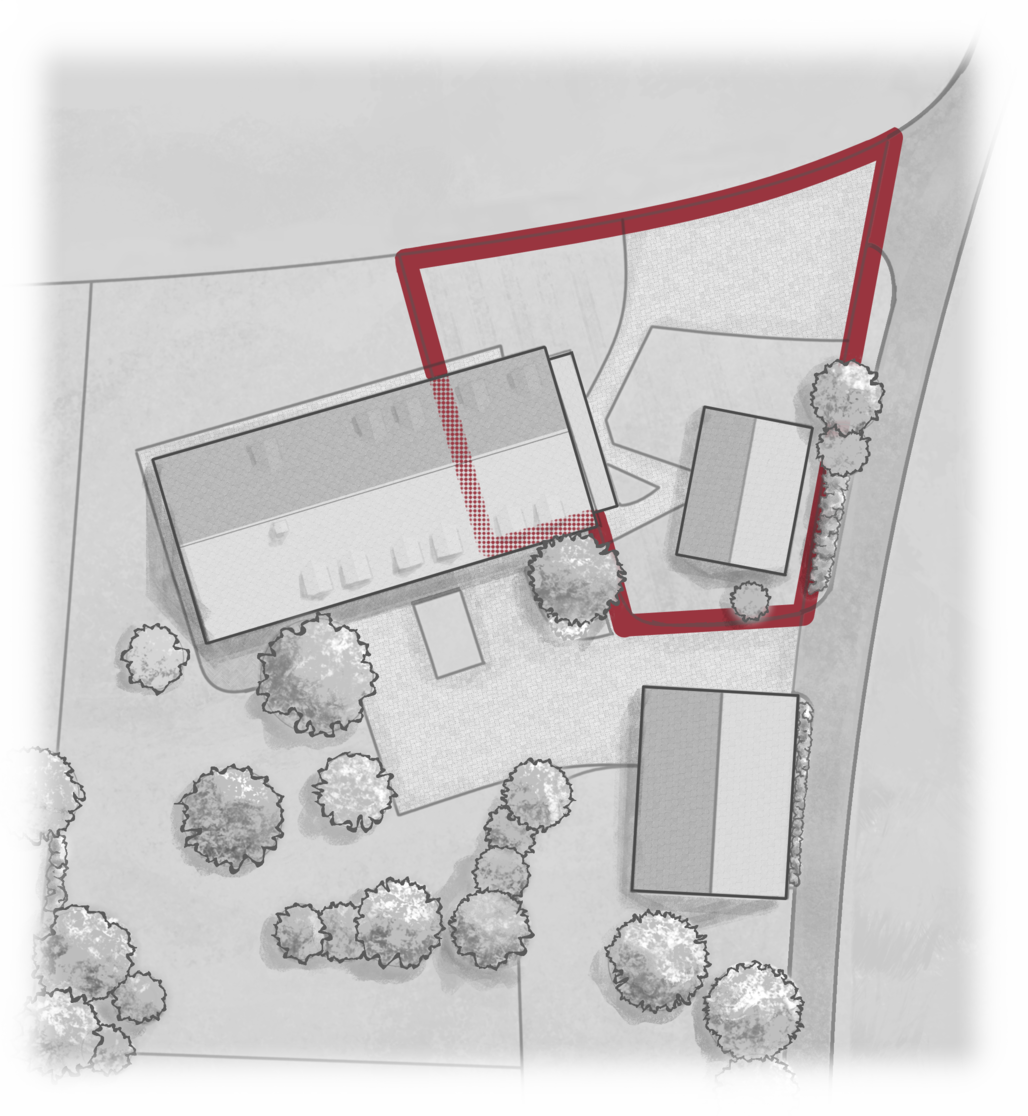
\includegraphics[width=\textwidth]{planek50.png}
%  \caption{Plánek Areálu zobrazující Penzion Spáleniště.}
%\end{figure}
%

\end{document}
